%Dokumentinnstillinger:---------------------------------
%Ved å google flitting kan du finne ut hva de forskjellige tingene her betyr, og hvordan du kan gjøre eventuelle endringer.
\documentclass[a4paper,11pt,norsk]{article}
\usepackage[utf8]{inputenc}
\usepackage{a4wide}
\usepackage{lmodern}
\usepackage[T1]{fontenc}
\usepackage{babel}
\usepackage{textcomp}

\setlength{\parindent}{0pt} 
\setlength{\parskip}{2ex}
\usepackage{fixltx2e}
\usepackage{amsmath}
\usepackage[pdftex, pdfborderstyle={/S/U/W 0}]{hyperref}
\usepackage{graphicx}
\usepackage[font=small,labelfont=bf]{caption}
\usepackage{tabularx}
\usepackage{multirow}
\usepackage{circuitikz}
% Adds seperation between two elements with a comma. Format: "    ,    ".
\newcommand{\comma}{\quad , \quad}
% Gives double underline under selected text.
\def\dunderline#1{\underline{\underline{#1}}}
% Faster way to make an equation that can be formatted with "&" to look nice.
\def\spliteq#1{\begin{equation}\begin{split}{#1}\end{split}\end{equation}\\}
%------------------------------------- End -------------------------------------

\begin{document}

%Headingdel:---------------------------------------------
\begin{minipage}[c]{0.15\textwidth}

\includegraphics[width=2.0cm]{elsys_pos_staaende_ntnu.png}
\end{minipage}
\begin{minipage}[c]{0.85\textwidth}

\renewcommand{\arraystretch}{1.7}
\large 
\begin{tabularx}{\textwidth}{|X|X|}
\hline
\multicolumn{2}{|l|}{} \\
\multicolumn{2}{|l|}{\huge \textbf{Designnotat 1}} \\
\multicolumn{2}{|l|}{}  \\
\hline
\multicolumn{2}{|l|}{Tittel: 
%Skriv inn tittel her:------------------------------------------
Enkle prinsipper for støyfjerning (AC-strøm)
} \\
\hline
\multicolumn{2}{|l|}{Forfattere: 
%Skriv inn forfattere her:--------------------------------------
Sindre Danielsen
} \\
\hline
%Skriv inn versjon og dato her her:-----------------------------
Versjon: 1.0 & Dato: 25.01.21
\\
\hline 
\end{tabularx}
\end{minipage}
\normalsize

%Automatisk generert innholdsfortegnelse:------------------

\setlength{\parskip}{0ex}
\renewcommand{\baselinestretch}{0.1}\normalsize
\tableofcontents
\renewcommand{\baselinestretch}{1.00}\normalsize
\setlength{\parskip}{2ex}
\rule{\textwidth}{1pt}

%Selve rapporten:----------------------------------------÷
\newpage
\section{Problembeskrivelse}
\label{sec:innledning}
Elektrisk støy er noe som forekommer, og ofte kan det være hensiktsmessing å fjerne det. Det ønskes da å utvikle et system 
\begin{figure}[htbp]
    \centering
    \begin{circuitikz} [american voltages, european resistors, baseline=(current bounding box.center)]
        \ctikzset { label/align = straight }
        \draw (2.5,2)
        to[short, -o] (4,2)
        to[short] (4.5,2)
        (4, 1.6) to [open,v=$\mathbf{x(t)}$] (4,0.4)
        % Bottom-left side
        (2.5,0) to[short, -o] (4,0)
        to[short] (4.5,0)
        % Top-right side
        (8.5,2) to[short, -o] (9,2)
        to[short] (10, 2)
        (9, 1.6) to [open,v=$\mathbf{\hat{s}(t)}$] (9,0.4)
        % Bottom-right side
        (10, 0) to[short, -o] (9,0)
        to[short] (8.5,0);
        
        % Nivåregulator
        \node[draw,minimum width=4cm,minimum height=3.8cm,anchor=south west] at (4.5,-0.90){$\mathbf{H}$};

        
    \end{circuitikz}
    \caption{Støyfjerning for vekselstrøm.}
  \label{fig:støyfjerner}
\end{figure}
\\
som tar inn et signal med støy $x(t)$ og gir oss ut et forbedret signal $\hat{s}(t)$. Funksjonen til støyfjerneren $H$ er å stoppe en unønsket frekvens ved bruk av et båndstopp filter.

\newpage
\section{Prinsipiell løsning}
\label{sec:prinsipielllosning}
Slik nevnt i seksjon~\ref{sec:innledning}, så kan støyfjerning løses ved bruk av et båndstopp filter. \\ Merk at: Optimalt ønskes det også en kaskadekobling av slike filter, som vi skal se på senere i denne seksjonen.
En krets som viser et enkelt båndstoppfilter er vist i
\begin{figure}[htbp]
    \centering
    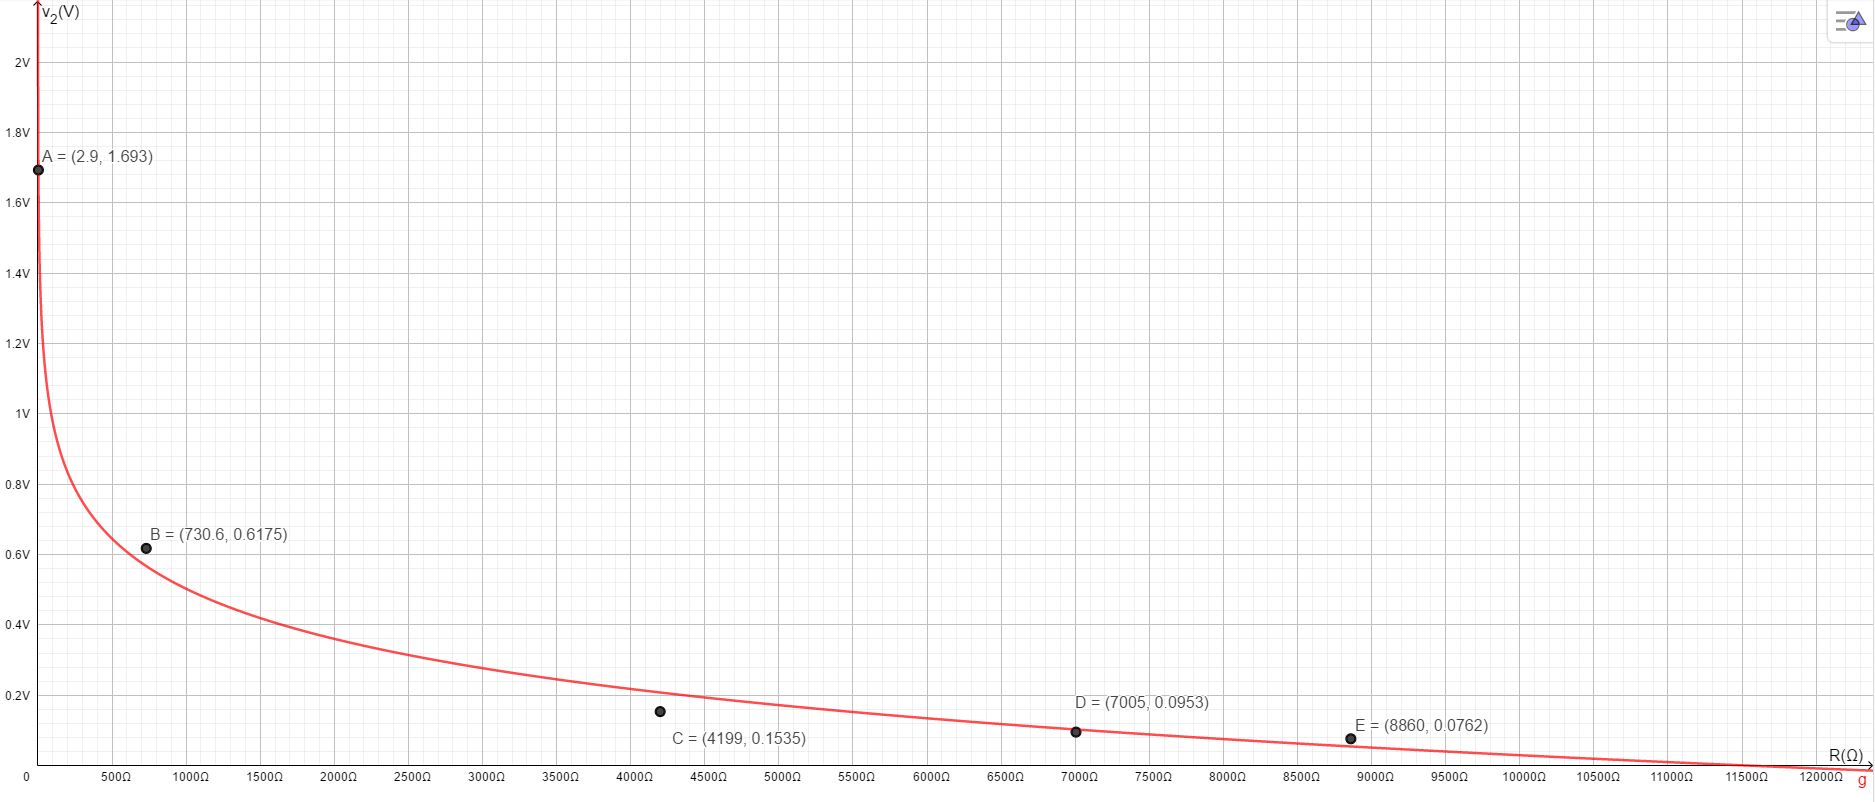
\includegraphics[width=1\textwidth]{graph}
    \begin{circuitikz} [american voltages, european resistors, european vresistors, baseline=(current bounding box.center)]
        \ctikzset { label/align = straight }
        \draw (0,0)
        to[short, o-] (2.5,0)
        to[R=$R_1$] (2.5, -2);
        \draw (2.5, -2)
        to[capacitor=$C_1$] (2.5, -4)
        ;
        \draw(2.5, -4)
        to[american inductor=$L_1$] (2.5, -6)
        (0, -2) to[open, v=$v_1$] (0,-4)
        (6, -3) to[open, v=$v_2$] (6,-5)
        ;
        \draw (2.5,-2) to[short, -o](6, -2)
        ;
        \draw (0,-6) to[short, o-o] (6,-6)
        ;
        \node[draw,dashed,minimum width=3.5cm,minimum height=8cm,anchor=south west] at (1,-7);
        
        
    \end{circuitikz}
    \caption{Båndstoppfilter}
    \label{fig:båndstoppfilter}
\end{figure}
\\
Hvis inngangsignalet $v_1$ inneholder støy, så vil utgangsignalet $v_2$ gi oss et båndstoppfilter gitt av resonansfrekvensen $w_0$, som er bestemt av kondenstaoren $C_1$ og  spolen $L_1$. Størrelsen på motstanden $R_1$ vil da gi signaldempningen i området rundt resonansfrekvensen. Denne signaldempninger kan vi utlede fra totalimpedansen gitt ved 
\\
$$Z = R_1 + j\omega L_1 - j \frac{1}{\omega C_1}$$
\begin{equation}
    \implies R =  Z - j\omega L_1 + j \frac{1}{\omega C_1}
\end{equation}
for $\omega \in \left<0,\infty\right> \backslash\{\omega_0\}$, der resonnansfrekvensen er gitt ved $w_0 = 2\pi f_0$.
\\
\\
Vi kaller støyets frekvens for $f_s$, så kan vi finne $C_1$ og $L_1$ ved å sette $\omega_0 = 2\pi f_s$, så vil \\ resonnansfrekvensen gi at
    $$2\pi f_s = \frac{1}{\sqrt{C_1 L_1}}$$
\begin{equation}
    \implies L_1 = \frac{1}{C (2 \pi f_s)^2} \comma C_1 = \frac{1}{L (2\pi f_s)^2}
\end{equation}\label{eq:resonnans}
som da betyr man kan selv velge verdien for enten $L_1$ eller $C_1$ og dermed rekne ut den andre. \\
\\
For at området i nærheten av $w_0$ skal påvirkes minst mulig av båndstoppfilteret, så kan vi kaskadekoble flere båndstoppfilter. Dette er vist ved
\begin{figure}[htbp]
    \centering
    
    \caption{Kaskadekobling med buffer som mellomledd.}
  \label{fig:kaskadekobling}
\end{figure}
\\

spenningsfallet over $R_1$ for  frekvensen $f_0$  bli størreblir  $R_1 = 5$k$\Omega$.

\newpage
\section{Konklusjon}
\label{sec:konklusjon}

\newpage

\begin{thebibliography}{9}

\bibitem{gn}
L. Lundheim: En generell nivåregulator \\
\textit{Teknisk notat 1, 2017}, Blackboard.
\bibitem{krets}
Lars Lundheim: Krets a) nivåregulator \\
\textit{Teknisk notat 1, 2017}, Blackboard.
\end{thebibliography}

\section{Vurdering av teksten}
\subsection{Generelt}
\begin{itemize}

\end{itemize}

\subsection{Teknikaliteter}
\begin{itemize}

\end{itemize}



\subsection{Kilder}
\begin{itemize}
    \item Kildene har et forståelig oppsett og blir brukt der de har behov for det. Nummereringen er også grei.
\end{itemize}

\subsection{Ønsker tilbakemelding på}

\newpage
%Bibliografi: Legg til flere elementer ved å legge til flere \bibitem:--------
\phantomsection

\appendix
%Tillegg. Flere tillegg legges til ved å lage flere sections:-----------------
\section{Utledning av $R_1$ og $R_2$}\label{attach:resistors}




\end{document}